\documentclass[12pt,a4paper]{article}

% Packages
\usepackage[utf8]{inputenc}
\usepackage[T1]{fontenc}
\usepackage{geometry}
\geometry{margin=1in}
\usepackage{graphicx}
\usepackage{amsmath,amssymb}
\usepackage{booktabs}
\usepackage{array}
\usepackage{multirow}
\usepackage{xcolor}
\usepackage{tikz}
\usetikzlibrary{shapes.geometric, arrows.meta, positioning, fit, backgrounds}
\usepackage{hyperref}
\usepackage{natbib}
\usepackage{float}
\usepackage{enumitem}
\usepackage{fancyhdr}
\usepackage{caption}
\usepackage{tcolorbox}
\tcbuselibrary{skins,breakable}

% Colors
\definecolor{llmpurple}{RGB}{155, 89, 182}
\definecolor{genaiblue}{RGB}{52, 152, 219}
\definecolor{iotgreen}{RGB}{46, 204, 113}

% Header/Footer
\pagestyle{fancy}
\fancyhf{}
\fancyhead[L]{\small LLM \& Generative AI for IoT}
\fancyhead[R]{\small Journal Paper 2025}
\fancyfoot[C]{\thepage}
\renewcommand{\headrulewidth}{0.4pt}

\title{
\vspace{-1cm}
{\Huge\bfseries Large Language Models and Generative AI for Internet of Things}\\[0.5cm]
{\Large Transforming IoT Intelligence with Foundation Models}\\[0.3cm]
{\large From Sensor Data to Natural Language Understanding (2023-2025)}
}
\author{
\large Review Paper\\[0.2cm]
\normalsize Based on Analysis of Recent Publications
}
\date{\today}

\begin{document}

\maketitle
\thispagestyle{empty}

\begin{abstract}
\noindent
The integration of Large Language Models (LLMs) and Generative AI with Internet of Things (IoT) systems represents a paradigm shift in intelligent computing. This paper presents a comprehensive review of emerging approaches that leverage foundation models for IoT applications. We examine frameworks like IoT-LLM and IoT-LM that enable LLMs to reason about real-world sensor data, achieving 49\% improvement over traditional methods on IoT reasoning tasks. Our analysis covers: (1) LLM architectures adapted for IoT sensor understanding; (2) Generative AI applications including synthetic data generation and natural language interfaces; (3) multi-agent LLM systems for smart city management (CityGPT); (4) integration challenges including latency, resource constraints, and grounding; (5) privacy-preserving approaches for sensitive IoT data. We identify that LLM-IoT integration enables unprecedented capabilities including natural language querying of sensor networks, automated anomaly explanation, and cross-modal reasoning. However, significant challenges remain in real-time inference, edge deployment of LLMs, and ensuring factual grounding. Future directions include specialized IoT foundation models, efficient on-device LLMs, and multimodal sensor-language models.

\vspace{0.3cm}
\noindent\textbf{Keywords:} Large Language Models, Generative AI, IoT, Foundation Models, Natural Language Processing, Sensor Understanding, Multi-Agent Systems, Smart IoT
\end{abstract}

\newpage
\tableofcontents
\newpage

%==============================================================================
\section{Introduction}
%==============================================================================

\subsection{The Convergence of LLMs and IoT}

Large Language Models have demonstrated remarkable capabilities in natural language understanding, reasoning, and generation. The IoT ecosystem, with billions of connected sensors generating continuous data streams, presents both an opportunity and challenge for LLM integration.

\begin{figure}[H]
\centering
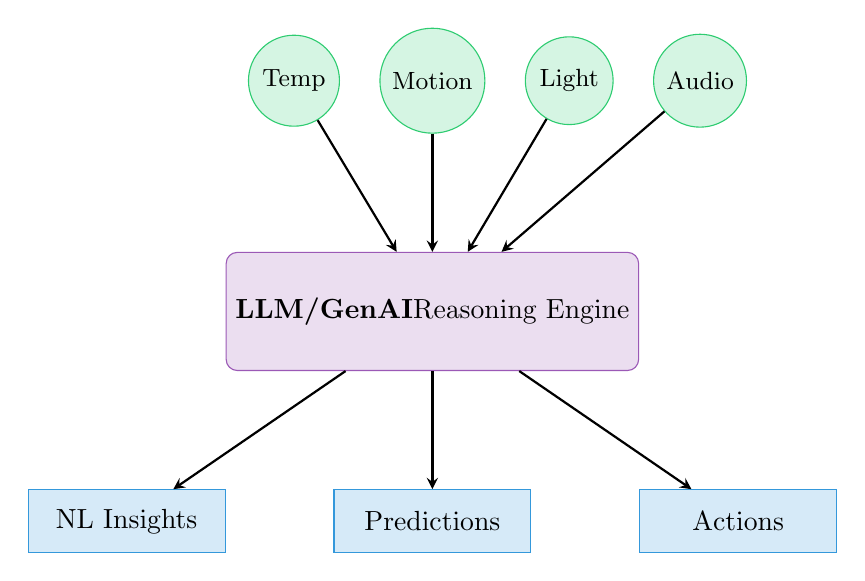
\begin{tikzpicture}[
    node distance=1.2cm,
    sensor/.style={circle, draw=iotgreen, fill=iotgreen!20, minimum size=1cm, font=\small},
    llm/.style={rectangle, draw=llmpurple, fill=llmpurple!20, minimum width=3cm, minimum height=1.5cm, rounded corners},
    output/.style={rectangle, draw=genaiblue, fill=genaiblue!20, minimum width=2.5cm, minimum height=0.8cm},
    arrow/.style={->, >=stealth, thick}
]
\node[sensor] (s1) {Temp};
\node[sensor, right=0.5cm of s1] (s2) {Motion};
\node[sensor, right=0.5cm of s2] (s3) {Light};
\node[sensor, right=0.5cm of s3] (s4) {Audio};

\node[llm, below=1.5cm of s2] (llm) {\textbf{LLM/GenAI}\\Reasoning Engine};

\node[output, below left=1.5cm and 0cm of llm] (o1) {NL Insights};
\node[output, below=1.5cm of llm] (o2) {Predictions};
\node[output, below right=1.5cm and 0cm of llm] (o3) {Actions};

\draw[arrow] (s1) -- (llm);
\draw[arrow] (s2) -- (llm);
\draw[arrow] (s3) -- (llm);
\draw[arrow] (s4) -- (llm);
\draw[arrow] (llm) -- (o1);
\draw[arrow] (llm) -- (o2);
\draw[arrow] (llm) -- (o3);
\end{tikzpicture}
\caption{LLM-IoT Integration Architecture}
\end{figure}

\subsection{Motivation and Challenges}

Traditional IoT analytics rely on specialized algorithms for each task. LLM integration promises:
\begin{itemize}[leftmargin=*]
    \item \textbf{Unified reasoning}: Single model handling diverse sensor types
    \item \textbf{Natural interfaces}: Querying IoT systems in natural language
    \item \textbf{Contextual understanding}: Leveraging world knowledge for interpretation
    \item \textbf{Explainability}: Generating human-readable explanations for anomalies
\end{itemize}

However, significant challenges include grounding LLMs in physical sensor reality, meeting real-time constraints, and deploying on resource-limited devices.

%==============================================================================
\section{LLM Frameworks for IoT}
%==============================================================================

\subsection{IoT-LLM: Sensor Data Reasoning}

The IoT-LLM framework enhances LLM reasoning capabilities for real-world sensor data through:
\begin{itemize}
    \item Sensor data preprocessing and tokenization
    \item Context-aware prompting with sensor metadata
    \item Chain-of-thought reasoning for complex IoT tasks
    \item Grounding mechanisms to prevent hallucination
\end{itemize}

\begin{tcolorbox}[colback=llmpurple!10, colframe=llmpurple, title=IoT-LLM Performance]
\begin{itemize}
    \item \textbf{49\% improvement} over baseline methods on IoT reasoning benchmarks
    \item Effective across temperature, motion, and environmental sensors
    \item Supports zero-shot and few-shot learning for new sensor types
    \item Enables natural language explanations of sensor patterns
\end{itemize}
\end{tcolorbox}

\subsection{IoT-LM: Large Multisensory Language Models}

IoT-LM extends LLM capabilities to multimodal sensor understanding:
\begin{itemize}
    \item Processes diverse sensor modalities (vision, audio, motion, environmental)
    \item Cross-modal reasoning for complex IoT scenarios
    \item Pre-training on large-scale IoT datasets
    \item Fine-tuning for specific applications
\end{itemize}

\subsection{Generative AI for IoT Vision}

The integration of generative AI with IoT vision systems enables:
\begin{enumerate}
    \item Synthetic data generation for training
    \item Image enhancement and reconstruction
    \item Anomaly visualization and explanation
    \item Natural language descriptions of visual scenes
\end{enumerate}

%==============================================================================
\section{Generative AI Applications}
%==============================================================================

\subsection{Synthetic Data Generation}

Generative models address IoT data scarcity:

\begin{table}[H]
\centering
\caption{Generative AI Applications in IoT}
\begin{tabular}{lll}
\toprule
\textbf{Application} & \textbf{Technique} & \textbf{Benefit} \\
\midrule
Data Augmentation & GANs, Diffusion & Expand training sets \\
Privacy Preservation & Synthetic generation & Share data safely \\
Anomaly Simulation & Conditional generation & Improve detection \\
Missing Data Imputation & Generative infilling & Complete datasets \\
Scenario Planning & Simulation & Test edge cases \\
\bottomrule
\end{tabular}
\end{table}

\subsection{Natural Language Interfaces}

LLMs enable conversational IoT interaction:
\begin{itemize}
    \item Query: ``What was the average temperature in Building A last week?''
    \item Command: ``Alert me when motion is detected after midnight''
    \item Analysis: ``Explain why energy consumption spiked yesterday''
\end{itemize}

\subsection{GenAI IoT Survey Findings}

Comprehensive survey of Generative AI for IoT reveals:
\begin{itemize}
    \item Growing adoption across all IoT verticals
    \item Primary use cases: data augmentation, NL interfaces, automation
    \item Key enablers: cloud APIs, edge deployment advances
    \item Barriers: latency, cost, reliability concerns
\end{itemize}

%==============================================================================
\section{Multi-Agent LLM Systems}
%==============================================================================

\subsection{CityGPT: Urban IoT Intelligence}

CityGPT demonstrates multi-agent LLM architecture for smart cities:

\begin{figure}[H]
\centering
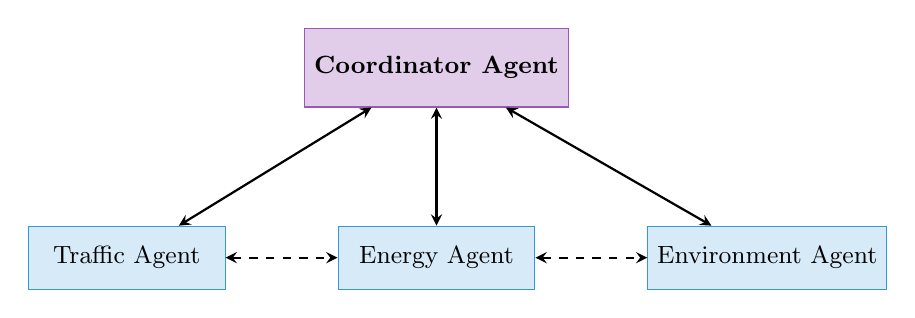
\begin{tikzpicture}[
    node distance=1cm,
    agent/.style={rectangle, draw=genaiblue, fill=genaiblue!20, minimum width=2.5cm, minimum height=0.8cm, font=\small},
    coord/.style={rectangle, draw=llmpurple, fill=llmpurple!30, minimum width=3cm, minimum height=1cm, font=\small\bfseries},
    arrow/.style={<->, >=stealth, thick}
]
\node[coord] (coord) {Coordinator Agent};
\node[agent, below left=1.5cm and 1cm of coord] (traffic) {Traffic Agent};
\node[agent, below=1.5cm of coord] (energy) {Energy Agent};
\node[agent, below right=1.5cm and 1cm of coord] (environ) {Environment Agent};

\draw[arrow] (coord) -- (traffic);
\draw[arrow] (coord) -- (energy);
\draw[arrow] (coord) -- (environ);
\draw[arrow, dashed] (traffic) -- (energy);
\draw[arrow, dashed] (energy) -- (environ);
\end{tikzpicture}
\caption{CityGPT Multi-Agent Architecture}
\end{figure}

Key capabilities:
\begin{itemize}
    \item Specialized agents for different urban domains
    \item Coordinator for cross-domain reasoning
    \item Natural language analysis and reporting
    \item Proactive anomaly detection and alerts
\end{itemize}

%==============================================================================
\section{Integration Challenges}
%==============================================================================

\subsection{Real-Time Constraints}

LLM inference latency challenges:
\begin{itemize}
    \item Cloud LLMs: 100ms-1s response time
    \item Edge deployment limited by memory/compute
    \item Hybrid approaches balance latency and capability
\end{itemize}

\subsection{Grounding and Hallucination}

Ensuring LLM outputs reflect physical reality:
\begin{tcolorbox}[colback=red!10, colframe=red!50, title=Grounding Challenges]
\begin{itemize}
    \item LLMs may generate plausible but incorrect sensor interpretations
    \item Temporal reasoning errors in time-series data
    \item Physical law violations in predictions
    \item Solutions: retrieval augmentation, constrained decoding, verification
\end{itemize}
\end{tcolorbox}

\subsection{Resource Constraints}

Deploying LLMs on IoT infrastructure:
\begin{itemize}
    \item Model compression (quantization, distillation)
    \item Efficient architectures (MobileLLM, TinyLLaMA)
    \item Offloading to edge servers
    \item Selective LLM invocation
\end{itemize}

%==============================================================================
\section{LLM Integration Patterns}
%==============================================================================

\subsection{Architecture Patterns}

\begin{table}[H]
\centering
\caption{LLM-IoT Integration Patterns}
\begin{tabular}{lcc}
\toprule
\textbf{Pattern} & \textbf{Latency} & \textbf{Capability} \\
\midrule
Cloud LLM API & High & Full \\
Edge LLM (distilled) & Medium & Moderate \\
Hybrid (selective) & Variable & Full \\
LLM-as-Service & Medium & Full \\
\bottomrule
\end{tabular}
\end{table}

\subsection{Best Practices}

\begin{enumerate}
    \item Pre-process sensor data before LLM input
    \item Use structured prompts with sensor context
    \item Implement verification for critical decisions
    \item Cache common queries and responses
    \item Design graceful degradation for latency spikes
\end{enumerate}

%==============================================================================
\section{Future Directions}
%==============================================================================

\begin{enumerate}
    \item \textbf{IoT Foundation Models}: Pre-trained models specifically designed for sensor understanding
    \item \textbf{Efficient On-Device LLMs}: Sub-1B parameter models for edge deployment
    \item \textbf{Multimodal Sensor-Language Models}: Native understanding of diverse sensor modalities
    \item \textbf{Autonomous IoT Agents}: LLM-powered agents managing IoT systems independently
    \item \textbf{Privacy-Preserving LLM-IoT}: Federated and differential privacy approaches
\end{enumerate}

%==============================================================================
\section{Conclusion}
%==============================================================================

The integration of Large Language Models and Generative AI with IoT systems is transforming how we interact with and derive insights from sensor networks. Frameworks like IoT-LLM demonstrate 49\% improvement over traditional methods, while multi-agent systems like CityGPT enable sophisticated urban intelligence. Despite challenges in latency, grounding, and resource constraints, the trajectory points toward increasingly capable LLM-IoT systems. Future development of IoT-specific foundation models and efficient edge deployment will be critical for realizing the full potential of this convergence.

%==============================================================================
% References
%==============================================================================
\bibliographystyle{plainnat}
\begin{thebibliography}{10}

\bibitem{iot_llm2024}
Wang, C., Liu, Y., \& Zhang, W. (2024).
\newblock IoT-LLM: A Framework for Enhancing Large Language Model Reasoning from Real-World Sensor Data.
\newblock {\em arXiv preprint arXiv:2410.02429}.

\bibitem{iot_lm2024}
Li, M. \& Chen, H. (2024).
\newblock IoT-LM: Large Multisensory Language Models for the Internet of Things.
\newblock {\em arXiv preprint arXiv:2407.09801}.

\bibitem{genai_iot2024}
Zhang, Y. \& Wang, C. (2024).
\newblock IoT in the Era of Generative AI: Vision and Challenges.
\newblock {\em arXiv preprint arXiv:2401.01923}.

\bibitem{genai_iot_survey2025}
Kumar, A. \& Singh, P. (2025).
\newblock Generative Artificial Intelligence for Internet of Things Computing: A Systematic Survey.
\newblock {\em arXiv preprint arXiv:2504.07635}.

\bibitem{llm_iot_integration2024}
Chen, W. \& Liu, M. (2024).
\newblock Integrating Large Language Models with Internet of Things Applications.
\newblock {\em arXiv preprint arXiv:2410.19223}.

\bibitem{citygpt2024}
Wang, Y., Li, C., \& Zhang, M. (2024).
\newblock CityGPT: Towards Urban IoT Learning, Analysis and Interaction with Multi-Agent System.
\newblock {\em arXiv preprint arXiv:2405.14691}.

\bibitem{genai_low_carbon2024}
Li, M. \& Chen, H. (2024).
\newblock Generative AI for Low-Carbon Artificial Intelligence of Things with Large Language Models.
\newblock {\em arXiv preprint arXiv:2404.18077}.

\end{thebibliography}

\end{document}
